\documentclass[8pt,aspectratio=169]{beamer}
\usetheme{Madrid}
\usepackage{graphicx}
\usepackage{booktabs}
\usepackage{adjustbox}
\usepackage{multicol}
\usepackage{amsmath}
\usepackage{amssymb}
\usepackage{tikz}
\usepackage{hyperref}
\usepackage{algorithm}
\usepackage{algorithmic}
\usepackage{colortbl}
\usepackage{pgfplots}
\pgfplotsset{compat=1.18}

% TikZ libraries for comics, diagrams, stakeholder maps
\usetikzlibrary{arrows.meta,positioning,shapes.callouts,shapes.geometric,decorations.pathreplacing}

% Color definitions
\definecolor{mlblue}{RGB}{0,102,204}
\definecolor{mlpurple}{RGB}{51,51,178}
\definecolor{mllavender}{RGB}{173,173,224}
\definecolor{mllavender2}{RGB}{193,193,232}
\definecolor{mllavender3}{RGB}{204,204,235}
\definecolor{mllavender4}{RGB}{214,214,239}
\definecolor{mlorange}{RGB}{255, 127, 14}
\definecolor{mlgreen}{RGB}{44, 160, 44}
\definecolor{mlred}{RGB}{214, 39, 40}
\definecolor{mlgray}{RGB}{127, 127, 127}
\definecolor{lightgray}{RGB}{240, 240, 240}
\definecolor{midgray}{RGB}{180, 180, 180}

% NEW COLORS for mini-lecture
\definecolor{dfteal}{RGB}{0,128,128}
\definecolor{dfred}{RGB}{180,30,30}

% Backward compatibility
\colorlet{MLPurple}{mlpurple}
\colorlet{MLBlue}{mlblue}
\colorlet{MLOrange}{mlorange}
\colorlet{MLGreen}{mlgreen}
\colorlet{MLRed}{mlred}
\colorlet{MLLavender}{mllavender}
\colorlet{MLGray}{mlgray}

% Theme colors (exact Madrid settings)
\setbeamercolor{palette primary}{bg=mllavender3,fg=mlpurple}
\setbeamercolor{palette secondary}{bg=mllavender2,fg=mlpurple}
\setbeamercolor{palette tertiary}{bg=mllavender,fg=white}
\setbeamercolor{palette quaternary}{bg=mlpurple,fg=white}
\setbeamercolor{structure}{fg=mlpurple}
\setbeamercolor{section in toc}{fg=mlpurple}
\setbeamercolor{subsection in toc}{fg=mlblue}
\setbeamercolor{title}{fg=mlpurple}
\setbeamercolor{frametitle}{fg=mlpurple,bg=mllavender3}
\setbeamercolor{block title}{bg=mllavender2,fg=mlpurple}
\setbeamercolor{block body}{bg=mllavender4,fg=black}
\setbeamertemplate{navigation symbols}{}
\setbeamertemplate{itemize items}[circle]
\setbeamertemplate{enumerate items}[default]
\setbeamersize{text margin left=5mm,text margin right=5mm}

% Footer
\setbeamertemplate{footline}{
  \leavevmode%
  \hbox{%
    \begin{beamercolorbox}[wd=.333333\paperwidth,ht=2.25ex,dp=1ex,center]{author in head/foot}%
      \usebeamerfont{author in head/foot}Methods and Algorithms
    \end{beamercolorbox}%
    \begin{beamercolorbox}[wd=.333333\paperwidth,ht=2.25ex,dp=1ex,center]{title in head/foot}%
      \usebeamerfont{title in head/foot}MSc Data Science
    \end{beamercolorbox}%
    \begin{beamercolorbox}[wd=.333333\paperwidth,ht=2.25ex,dp=1ex,right]{date in head/foot}%
      \usebeamerfont{date in head/foot}\insertframenumber{} / \inserttotalframenumber\hspace*{2ex}
    \end{beamercolorbox}}%
  \vskip0pt%
}

\newcommand{\bottomnote}[1]{%
\vfill
\vspace{-2mm}
\textcolor{mllavender2}{\rule{\textwidth}{0.4pt}}
\vspace{1mm}
\footnotesize
\textbf{#1}
}

\newenvironment{compactlist}{%
  \begin{itemize}%
    \setlength{\itemsep}{2pt}%
    \setlength{\parskip}{0pt}%
    \setlength{\parsep}{0pt}%
}{%
  \end{itemize}%
}

\newcommand{\highlight}[1]{\textcolor{mlorange}{\textbf{#1}}}
\newcommand{\mathbold}[1]{\boldsymbol{#1}}

\title[t-SNE Full Lecture]{t-SNE: Visualizing High-Dimensional Data}
\subtitle{Preserving Neighborhoods in Two Dimensions}
\author{Methods \& Algorithms}
\date{MSc Data Science -- Spring 2026}

\begin{document}

%% ================================================================
%% INTRO ZONE (Slides 1-5, NO formulas)
%% ================================================================

%% SLIDE 1: Title Page
\begin{frame}[plain]
\titlepage
\end{frame}

%% SLIDE 2: Opening TikZ Comic
\begin{frame}[t]{How Do You Spot a Market Crash in 100 Variables?}
\begin{columns}[T]
\column{0.55\textwidth}
\small
\textbf{The Visualization Challenge}
\begin{compactlist}
\item You monitor 100 risk indicators: VIX, credit spreads, correlations, order flow\ldots
\item A dashboard with 100 time series is overwhelming -- you cannot see the ``big picture''
\item What if you could collapse all 100 signals into a single 2D map?
\end{compactlist}

\begin{block}{The Question}
\scriptsize Can we project 100D data into 2D so that similar market states cluster together -- revealing regimes, anomalies, and transitions?
\end{block}

\column{0.42\textwidth}
\vspace{2mm}
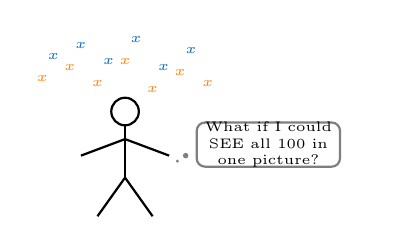
\begin{tikzpicture}[scale=0.7]
  % Analyst stick figure
  \draw[thick] (1.5,3.5) circle (0.25);
  \draw[thick] (1.5,3.25) -- (1.5,2.3);
  \draw[thick] (1.5,3.0) -- (0.7,2.7);
  \draw[thick] (1.5,3.0) -- (2.3,2.7);
  \draw[thick] (1.5,2.3) -- (1.0,1.6);
  \draw[thick] (1.5,2.3) -- (2.0,1.6);
  % Wave of numbers/variables
  \foreach \x/\y in {0.2/4.5, 0.7/4.7, 1.2/4.4, 1.7/4.8, 2.2/4.3, 2.7/4.6} {
    \node[font=\tiny, mlblue] at (\x,\y) {$x$};
  }
  \foreach \x/\y in {0.0/4.1, 0.5/4.3, 1.0/4.0, 1.5/4.4, 2.0/3.9, 2.5/4.2, 3.0/4.0} {
    \node[font=\tiny, mlorange] at (\x,\y) {$x$};
  }
  % Thought bubble
  \draw[mlgray, thick, rounded corners=3pt] (2.8,2.5) rectangle (5.4,3.3);
  \node[font=\tiny, text width=2.3cm, align=center] at (4.1,2.9) {What if I could SEE all 100 in one picture?};
  \fill[mlgray] (2.6,2.7) circle (0.05);
  \fill[mlgray] (2.45,2.6) circle (0.03);
\end{tikzpicture}
\end{columns}

\bottomnote{van der Maaten \& Hinton (2008) introduced t-SNE -- now the standard tool for visualizing high-dimensional data}
\end{frame}

%% SLIDE 3: Learning Objectives
\begin{frame}[t]{Learning Objectives}
\begin{columns}[T]
\column{0.95\textwidth}
\small
After this lecture, you will be able to:

\vspace{3mm}
\begin{enumerate}
\setlength{\itemsep}{6pt}
\item \highlight{Derive} t-SNE's KL divergence objective and understand the role of the gradient
\item \highlight{Analyze} how perplexity controls the balance between local and global structure
\item \highlight{Evaluate} t-SNE's limitations compared to PCA and UMAP
\item \highlight{Apply} t-SNE to detect market regimes and spot financial anomalies
\end{enumerate}

\vspace{3mm}
\begin{block}{Prerequisites}
\scriptsize Probability (conditional distributions), PCA basics (from the PCA lecture), Python with scikit-learn.
\end{block}
\end{columns}

\bottomnote{All learning objectives target Bloom's level 4+ (derive, analyze, evaluate, apply)}
\end{frame}

%% SLIDE 4: What Is t-SNE in Plain English?
\begin{frame}[t]{What Is t-SNE in Plain English?}
\begin{columns}[T]
\column{0.55\textwidth}
\small
\textbf{The Dinner Guests Analogy}
\begin{compactlist}
\item Imagine seating 200 dinner guests at round tables
\item Friends should sit together; strangers should be at different tables
\item t-SNE does this with data: \highlight{convert distances to ``friendship probabilities''} in high-D, then find a 2D seating plan that preserves those friendships
\end{compactlist}

\begin{block}{Core Idea}
\scriptsize If two points are close in 100D (high probability of being neighbors), they must land close in 2D. If they are far, push them apart.
\end{block}

\column{0.42\textwidth}
\vspace{2mm}
\footnotesize
\fcolorbox{mlpurple}{mllavender4}{\parbox{0.85\columnwidth}{%
\textbf{t-SNE in 3 Steps:}

\vspace{2mm}
\textbf{1.} Compute pairwise ``similarity'' in high-D (Gaussian kernel)

\vspace{2mm}
\textbf{2.} Initialize random 2D layout

\vspace{2mm}
\textbf{3.} Iteratively adjust 2D positions to match high-D similarities (minimize KL divergence)

\vspace{2mm}
\textit{``t''} = Student-t kernel in low-D
}}
\end{columns}

\bottomnote{t-SNE is for visualization only -- the 2D coordinates are not features for downstream models}
\end{frame}

%% SLIDE 5: Why Not Just Use PCA?
\begin{frame}[t]{Why Not Just Use PCA?}
\begin{columns}[T]
\column{0.95\textwidth}
\small
\textbf{PCA's Linear Limitation}

\vspace{2mm}
\begin{compactlist}
\item Recall the Swiss roll from the PCA lecture: PCA projects onto a flat plane, destroying the manifold structure
\item Points that are \emph{far apart} on the surface end up \emph{close together} after PCA projection
\item Colors interleave instead of forming clean clusters
\end{compactlist}

\vspace{2mm}
\footnotesize
\begin{tabular}{@{}l l l@{}}
\toprule
& \textbf{PCA} & \textbf{t-SNE} \\
\midrule
\rowcolor{mllavender4}
Swiss roll & Flattens, colors mix & Unrolls, colors separate \\
Preserves & Global variance & Local neighborhoods \\
\rowcolor{mllavender4}
Best for & Linear structure & Non-linear manifolds \\
\bottomrule
\end{tabular}

\vspace{2mm}
\begin{block}{Key Insight}
\scriptsize PCA captures directions of maximum \emph{spread}. t-SNE captures who is \emph{near} whom. For discovering clusters in complex data, neighborhoods matter more.
\end{block}
\end{columns}

\bottomnote{PCA is a global method (variance); t-SNE is a local method (neighborhoods) -- they answer different questions}
\end{frame}

%% ================================================================
%% CORE ZONE -- METHOD (Slides 6-14)
%% ================================================================

%% SLIDE 6: Full Chart -- Swiss Roll t-SNE
\begin{frame}[t]{How Does t-SNE Preserve Neighborhoods?}
\begin{center}

\includegraphics[width=0.65\textwidth]{05b_tsne_swiss_roll/chart.pdf}
\end{center}

\bottomnote{t-SNE ``unrolls'' the Swiss roll -- points near each other on the surface stay near each other in 2D}
\end{frame}

%% SLIDE 7: Definition Block -- High-D Similarities
\begin{frame}[t]{Step 1: Compute Pairwise Similarities in High-D}
\begin{columns}[T]
\column{0.95\textwidth}
\small

\vspace{1mm}
\begin{block}{Conditional Probability (Gaussian Kernel)}
\[
p_{j|i} = \frac{\exp\!\bigl(-\|x_i - x_j\|^2 \,/\, 2\sigma_i^2\bigr)}{\sum_{k \neq i}\exp\!\bigl(-\|x_i - x_k\|^2 \,/\, 2\sigma_i^2\bigr)}
\]
\end{block}

\vspace{1mm}
\begin{compactlist}
\item $p_{j|i}$: probability that $x_i$ would pick $x_j$ as a neighbor
\item $\sigma_i$: bandwidth, set automatically so each point has \highlight{perplexity} effective neighbors
\item Symmetrize: $p_{ij} = (p_{j|i} + p_{i|j}) \,/\, 2n$
\item Closer points $\Rightarrow$ higher $p_{ij}$. Far points $\Rightarrow$ $p_{ij} \approx 0$.
\end{compactlist}

\begin{block}{Intuition}
\scriptsize The Gaussian kernel converts Euclidean distances into ``how likely is $x_j$ to be a neighbor of $x_i$?'' -- points within $\sigma_i$ get high probability, distant points get near zero.
\end{block}
\end{columns}

\bottomnote{Each point gets its own $\sigma_i$ -- dense regions use small $\sigma$, sparse regions use large $\sigma$}
\end{frame}

%% SLIDE 8: Definition Block -- Low-D Similarities
\begin{frame}[t]{Step 2: Similarities in Low-D (Student-t Kernel)}
\begin{columns}[T]
\column{0.95\textwidth}
\small

\vspace{1mm}
\begin{block}{Student-t Kernel in 2D}
\[
q_{ij} = \frac{(1 + \|y_i - y_j\|^2)^{-1}}{\sum_{k \neq l}(1 + \|y_k - y_l\|^2)^{-1}}
\]
\end{block}

\vspace{1mm}
\begin{compactlist}
\item $y_i, y_j$: positions in the 2D embedding
\item The denominator normalizes across all pairs so $q_{ij}$ sums to 1
\item \highlight{Why Student-t?} Its heavy tails give moderate-distance pairs more room
\item Unlike the Gaussian, Student-t does not decay as fast -- this prevents crowding
\end{compactlist}

\begin{block}{Goal}
\scriptsize Make $q_{ij}$ match $p_{ij}$ as closely as possible by adjusting the 2D coordinates $y_i$.
\end{block}
\end{columns}

\bottomnote{Student-t with 1 degree of freedom = Cauchy distribution -- heavier tails than Gaussian, which is the key to avoiding the crowding problem}
\end{frame}

%% SLIDE 9: KL Divergence
\begin{frame}[t]{Step 3: Minimize KL Divergence}
\begin{columns}[T]
\column{0.95\textwidth}
\small

\vspace{1mm}
\begin{block}{t-SNE Objective Function}
\[
\text{KL}(P\|Q) = \sum_i \sum_j p_{ij} \log \frac{p_{ij}}{q_{ij}}
\]
\end{block}

\vspace{1mm}
\textbf{What the KL divergence penalizes:}
\begin{compactlist}
\item \highlight{High $p_{ij}$, low $q_{ij}$}: nearby points in high-D that are far apart in 2D $\Rightarrow$ \textbf{large penalty}
\item \highlight{Low $p_{ij}$, high $q_{ij}$}: distant points in high-D that end up close in 2D $\Rightarrow$ \textbf{small penalty}
\item This asymmetry means: t-SNE is very good at keeping neighbors together, less strict about pushing non-neighbors apart
\end{compactlist}

\begin{block}{Consequence}
\scriptsize t-SNE reliably preserves local structure (clusters). It does \emph{not} reliably preserve global structure (distances between clusters).
\end{block}
\end{columns}

\bottomnote{KL divergence is asymmetric -- $\text{KL}(P\|Q) \neq \text{KL}(Q\|P)$. The choice $\text{KL}(P\|Q)$ prioritizes keeping nearby points together.}
\end{frame}

%% SLIDE 10: The Crowding Problem
\begin{frame}[t]{The Crowding Problem: Why Student-t?}
\begin{columns}[T]
\column{0.47\textwidth}
\small
\textbf{Gaussian in Low-D: Crowding}
\begin{compactlist}
\item In high-D, there is room for many equidistant neighbors (surface of a hypersphere grows as $r^{d-1}$)
\item In 2D, there is much less room
\item With a Gaussian kernel, moderate-distance points get squashed into the center
\item Result: one big blob instead of distinct clusters
\end{compactlist}

\column{0.50\textwidth}
\small
\textbf{Student-t in Low-D: Solution}
\begin{compactlist}
\item Heavy tails allow moderate-distance pairs to be further apart in 2D
\item Tight clusters form for true neighbors
\item Clear gaps between clusters
\item The ``t'' in t-SNE stands for this Student-t trick
\end{compactlist}

\vspace{2mm}
\begin{block}{Example}
\scriptsize 10 equidistant points on a circle in 100D: Gaussian mapping $\rightarrow$ overlapping blob. Student-t mapping $\rightarrow$ evenly spaced ring.
\end{block}
\end{columns}

\bottomnote{The crowding problem is why early SNE (2002, Gaussian in both spaces) produced poor visualizations -- the Student-t fix (2008) was the breakthrough}
\end{frame}

%% SLIDE 11: Three Charts Side-by-Side -- Perplexity
\begin{frame}[t]{What Does Perplexity Do?}
\begin{center}

\includegraphics[width=0.30\textwidth]{04a_tsne_perplexity_5/chart.pdf}\hfill

\includegraphics[width=0.30\textwidth]{04b_tsne_perplexity_30/chart.pdf}\hfill

\includegraphics[width=0.30\textwidth]{04c_tsne_perplexity_100/chart.pdf}
\end{center}

\vspace{1mm}
\small
\begin{compactlist}
\item \textbf{Left} (perplexity=5): very local focus, many small fragments
\item \textbf{Center} (perplexity=30): balanced -- the sklearn default
\item \textbf{Right} (perplexity=100): global focus, clusters may merge
\end{compactlist}

\bottomnote{Perplexity $\approx$ effective number of neighbors. Always try at least 3 values before drawing conclusions.}
\end{frame}

%% SLIDE 12: Perplexity Guidelines
\begin{frame}[t]{Perplexity Guidelines}
\begin{columns}[T]
\column{0.95\textwidth}
\small

\vspace{1mm}
\footnotesize
\begin{tabular}{@{}l l l@{}}
\toprule
\textbf{Perplexity Range} & \textbf{Behavior} & \textbf{When to Use} \\
\midrule
\rowcolor{mllavender4}
5--10 & Very local, risk of fragmentation & Small datasets ($n < 100$) \\
20--30 & Balanced local/global (sklearn default) & General purpose \\
\rowcolor{mllavender4}
50--100 & More global, smoother layout & Large datasets ($n > 5{,}000$) \\
$> 100$ & Over-smoothed, clusters merge & Rarely useful \\
\bottomrule
\end{tabular}

\vspace{3mm}
\textbf{Rules of Thumb:}
\begin{compactlist}
\item Perplexity should be smaller than $n/3$ (where $n$ = number of points)
\item Always try at least 3 values (e.g.\ 5, 30, 100) before interpreting
\item If patterns change drastically with perplexity, they are artifacts -- not real structure
\end{compactlist}

\begin{block}{Technical Detail}
\scriptsize Perplexity sets $\sigma_i$ via binary search so that the entropy of $p_{j|i}$ equals $\log_2(\text{perplexity})$. Higher perplexity = larger $\sigma_i$ = more neighbors considered.
\end{block}
\end{columns}

\bottomnote{Wattenberg et al.\ (2016) ``How to Use t-SNE Effectively'' -- interactive demo and essential reading}
\end{frame}

%% SLIDE 13: Caveats
\begin{frame}[t]{t-SNE Caveats: What You Cannot Infer}
\begin{columns}[T]
\column{0.47\textwidth}
\small
\textbf{What IS Meaningful}
\begin{compactlist}
\item Points within a cluster are truly similar in high-D
\item The existence of clusters (local structure) is real
\item Relative positions \emph{within} a cluster are approximately preserved
\end{compactlist}

\column{0.50\textwidth}
\small
\textbf{What is NOT Meaningful}
\begin{compactlist}
\item \highlight{Cluster sizes}: a big cluster is not ``more spread out'' in high-D
\item \highlight{Inter-cluster distances}: a gap between clusters means nothing about true distance
\item \highlight{Axis orientation}: axes are random (no ``x-axis = feature 1'')
\item \highlight{Reproducibility}: different random seeds produce different layouts
\end{compactlist}
\end{columns}

\vspace{3mm}
\begin{block}{Golden Rule}
\scriptsize t-SNE is for \textbf{exploration}, not measurement. Use it to generate hypotheses, then test them with statistical methods.
\end{block}

\bottomnote{Never report ``cluster A is closer to cluster B than to cluster C'' based on a t-SNE plot -- that distance is meaningless}
\end{frame}

%% SLIDE 14: Full Chart -- Cluster Preservation
\begin{frame}[t]{How Does Cluster Preservation Compare?}
\begin{center}

\includegraphics[width=0.65\textwidth]{06c_tsne_cluster_projection/chart.pdf}
\end{center}

\bottomnote{t-SNE separates clusters that PCA merges -- this is its key advantage for visualization of non-linear structure}
\end{frame}

%% ================================================================
%% CORE ZONE -- SOLUTION (Slides 15-19)
%% ================================================================

%% SLIDE 15: Market Regime Detection
\begin{frame}[t]{Market Regime Detection with t-SNE}
\begin{columns}[T]
\column{0.47\textwidth}
\small
\textbf{The Setup}
\begin{compactlist}
\item Collect daily return vectors of 50 stocks over 5 years
\item Each day is a point in 50D (one dimension per stock)
\item Run t-SNE to project into 2D
\item Color points by date
\end{compactlist}

\column{0.50\textwidth}
\small
\textbf{What You See}
\begin{compactlist}
\item Clusters = \highlight{market regimes} (bull, bear, crisis)
\item 2008 trading days cluster together, separate from 2005 days
\item Transitions between regimes appear as bridges between clusters
\item Outlier days (flash crashes) appear isolated
\end{compactlist}
\end{columns}

\vspace{2mm}
\begin{block}{Interpretation}
\scriptsize The cross-sectional return pattern on crisis days is similar to other crisis days but different from calm days. t-SNE makes this visible.
\end{block}

\bottomnote{Regime detection via t-SNE complements hidden Markov models -- it provides visual confirmation and exploratory insight}
\end{frame}

%% SLIDE 16: Anomaly Detection
\begin{frame}[t]{Anomaly Detection: Spotting Outliers Visually}
\begin{columns}[T]
\column{0.95\textwidth}
\small
\textbf{Outliers in the t-SNE Map}

\vspace{2mm}
\begin{compactlist}
\item Points far from any cluster in the 2D embedding are potential anomalies
\item In finance: rogue trading days, flash crashes, data errors, or unprecedented market events
\item t-SNE does not label anomalies -- it makes them \highlight{visible} for human investigation
\end{compactlist}

\vspace{2mm}
\footnotesize
\begin{tabular}{@{}l l@{}}
\toprule
\textbf{Outlier Pattern} & \textbf{Possible Cause} \\
\midrule
\rowcolor{mllavender4}
Isolated point far from all clusters & Unprecedented event (e.g.\ COVID crash day) \\
Small cluster of 2--3 points & Repeated anomaly (e.g.\ flash crash pattern) \\
\rowcolor{mllavender4}
Point between two clusters & Regime transition day \\
\bottomrule
\end{tabular}

\vspace{2mm}
\begin{block}{Complementary Approach}
\scriptsize Use t-SNE for visual exploration, then confirm with statistical tests (Mahalanobis distance, isolation forest).
\end{block}
\end{columns}

\bottomnote{t-SNE is a complement to, not a replacement for, statistical outlier detection methods}
\end{frame}

%% SLIDE 17: UMAP
\begin{frame}[t]{UMAP: The Modern Alternative}
\begin{columns}[T]
\column{0.95\textwidth}
\small

\vspace{1mm}
\footnotesize
\begin{tabular}{@{}l c c@{}}
\toprule
\textbf{Property} & \textbf{t-SNE} & \textbf{UMAP} \\
\midrule
\rowcolor{mllavender4}
Speed & Slow ($O(n^2)$, Barnes-Hut: $O(n \log n)$) & Fast ($O(n^{1.14})$) \\
Global structure & Poorly preserved & Better preserved \\
\rowcolor{mllavender4}
Reproducibility & Random (set seed) & More deterministic \\
New point projection & Not supported & Supported (transform) \\
\rowcolor{mllavender4}
Theory & KL divergence & Cross-entropy on fuzzy sets \\
Clusters & Excellent & Excellent \\
\bottomrule
\end{tabular}

\vspace{3mm}
\begin{compactlist}
\item UMAP (McInnes et al., 2018) follows the same idea: find a 2D layout preserving neighborhoods
\item \highlight{Key advantage}: UMAP scales to millions of points and preserves more global structure
\item \highlight{Key similarity}: both are for visualization and exploration -- same caveats apply
\end{compactlist}

\begin{block}{When to Choose UMAP over t-SNE}
\scriptsize Use UMAP when $n > 10{,}000$, when you need to project new data, or when global structure matters.
\end{block}
\end{columns}

\bottomnote{UMAP is not a strict upgrade -- t-SNE may produce tighter local clusters. Try both and compare.}
\end{frame}

%% SLIDE 18: Decision Framework -- Chart + Table
\begin{frame}[t]{t-SNE vs PCA vs UMAP: Decision Framework}
\begin{columns}[T]
\column{0.55\textwidth}

\includegraphics[width=\textwidth]{07_decision_flowchart/chart.pdf}

\column{0.42\textwidth}
\small
\footnotesize
\begin{tabular}{@{}l c c c@{}}
\toprule
& \textbf{PCA} & \textbf{t-SNE} & \textbf{UMAP} \\
\midrule
\rowcolor{mllavender4}
Speed & +++ & + & ++ \\
Global & +++ & + & ++ \\
\rowcolor{mllavender4}
Local & + & +++ & +++ \\
Interp. & +++ & -- & -- \\
\rowcolor{mllavender4}
Reprod. & +++ & + & ++ \\
\bottomrule
\end{tabular}

\vspace{2mm}
\scriptsize \textbf{Decision rule:}

Need features? $\rightarrow$ PCA

Need clusters? $\rightarrow$ t-SNE or UMAP

$n > 10$K? $\rightarrow$ UMAP
\end{columns}

\bottomnote{In practice, run PCA first (reduce to 30--50D), then t-SNE or UMAP on the PCA output for best results}
\end{frame}

%% SLIDE 19: The t-SNE Gradient
\begin{frame}[t]{The t-SNE Gradient}
\begin{columns}[T]
\column{0.95\textwidth}
\small

\vspace{1mm}
\begin{block}{Gradient of the KL Divergence}
\[
\frac{\partial C}{\partial y_i} = 4\sum_j (p_{ij} - q_{ij})(y_i - y_j)\bigl(1 + \|y_i - y_j\|^2\bigr)^{-1}
\]
\end{block}

\vspace{1mm}
\textbf{Interpreting the Gradient:}
\begin{compactlist}
\item When $p_{ij} > q_{ij}$: points are neighbors in high-D but too far in 2D $\Rightarrow$ \highlight{attractive force} pulls $y_i$ toward $y_j$
\item When $p_{ij} < q_{ij}$: points are not neighbors but too close in 2D $\Rightarrow$ \highlight{repulsive force} pushes $y_i$ away from $y_j$
\item The $(1 + \|y_i - y_j\|^2)^{-1}$ term modulates the force: nearby pairs feel stronger forces
\end{compactlist}

\begin{block}{Optimization}
\scriptsize t-SNE uses gradient descent with momentum. Early exaggeration (multiplying $p_{ij}$ by 4 for the first 250 iterations) helps form initial clusters.
\end{block}
\end{columns}

\bottomnote{The gradient has a physical interpretation: each point is pulled by its neighbors and pushed by non-neighbors, like a spring system}
\end{frame}

%% ================================================================
%% CLOSING ZONE (Slides 20-25)
%% ================================================================

%% SLIDE 20: When to Use t-SNE
\begin{frame}[t]{When to Use t-SNE --- and When Not To}
\begin{columns}[T]
\column{0.47\textwidth}
\small
\textbf{\textcolor{mlgreen}{Pros}}
\begin{compactlist}
\item Reveals clusters invisible to linear methods
\item Handles non-linear manifolds (Swiss roll, clusters)
\item Produces visually stunning, interpretable 2D plots
\item Standard tool -- reviewers expect it
\end{compactlist}

\column{0.50\textwidth}
\small
\textbf{\textcolor{mlred}{Cons}}
\begin{compactlist}
\item Slow: $O(n^2)$ naive, $O(n \log n)$ with Barnes-Hut
\item Non-reproducible without fixed seed
\item Cannot project new points (no \texttt{transform})
\item Uninterpretable axes and distances
\end{compactlist}
\end{columns}

\vspace{3mm}
\begin{block}{Rule of Thumb}
\scriptsize Use t-SNE for exploratory visualization of $n < 10{,}000$ points. For larger datasets or when you need projection, use UMAP.
\end{block}

\bottomnote{t-SNE is the most-cited visualization method in ML -- but it is also the most misinterpreted. Know the caveats.}
\end{frame}

%% SLIDE 21: t-SNE vs Logistic Regression
\begin{frame}[t]{t-SNE vs Logistic Regression Feature Space}
\begin{columns}[T]
\column{0.95\textwidth}
\small
\textbf{When PCA + Logistic Regression Fails}

\vspace{2mm}
\begin{compactlist}
\item Logistic regression draws a linear boundary in feature space
\item If classes are not linearly separable after PCA projection, LR fails
\item \highlight{t-SNE visualization shows why}: classes that overlap in PCA's 2D view may form distinct clusters in t-SNE's 2D view
\item This tells you the signal exists -- you just need a non-linear model (SVM, random forest, neural net)
\end{compactlist}

\vspace{2mm}
\footnotesize
\begin{tabular}{@{}l l l@{}}
\toprule
\textbf{Scenario} & \textbf{PCA 2D} & \textbf{t-SNE 2D} \\
\midrule
\rowcolor{mllavender4}
Linear classes & Separated & Separated \\
Non-linear classes & Overlapping & Separated \\
\rowcolor{mllavender4}
No structure & Overlapping & Overlapping \\
\bottomrule
\end{tabular}

\begin{block}{Diagnostic Use}
\scriptsize If t-SNE shows clusters but PCA does not, your data has non-linear structure. Switch from linear models to non-linear ones.
\end{block}
\end{columns}

\bottomnote{t-SNE as a diagnostic: it tells you whether the signal is there, even if your current model cannot capture it}
\end{frame}

%% SLIDE 22: Hands-on Code (fragile)
\begin{frame}[fragile,t]{Hands-on: Detect Market Regimes}
\begin{columns}[T]
\column{0.95\textwidth}
\small

\vspace{2mm}
\begin{verbatim}
from sklearn.manifold import TSNE
from sklearn.preprocessing import StandardScaler
import numpy as np

np.random.seed(42)
# Simulate 500 trading days x 50 stocks
returns = np.random.randn(500, 50) * 0.02

X = StandardScaler().fit_transform(returns)

# Try 3 perplexities
for perp in [5, 30, 100]:
    emb = TSNE(n_components=2, perplexity=perp,
               random_state=42, n_iter=1000).fit_transform(X)
    print(f"Perplexity={perp}: shape={emb.shape}")
\end{verbatim}

\vspace{1mm}
\scriptsize Full notebook: \texttt{notebooks/L05\_tsne.ipynb}
\end{columns}

\bottomnote{Always set \texttt{random\_state} for reproducibility and \texttt{n\_iter=1000} (minimum) for convergence}
\end{frame}

%% SLIDE 23: Key Takeaways
\begin{frame}[t]{Key Takeaways}
\begin{columns}[T]
\column{0.47\textwidth}
\small
\textbf{Concepts}
\begin{compactlist}
\item t-SNE minimizes KL divergence between high-D and low-D similarity distributions
\item Student-t kernel in low-D solves the crowding problem
\item Perplexity controls local vs.\ global balance
\item Cluster sizes and distances are meaningless
\end{compactlist}

\column{0.50\textwidth}
\small
\textbf{Practice}
\begin{compactlist}
\item Always try 3+ perplexity values before interpreting
\item Do not read distances or cluster sizes from the plot
\item Use for exploration only, not as model features
\item Consider UMAP for speed and global structure
\end{compactlist}
\end{columns}

\vspace{4mm}
\begin{block}{One-Sentence Summary}
\scriptsize t-SNE converts high-D distances to neighbor probabilities, then finds a 2D layout that preserves those neighborhoods -- revealing clusters invisible to linear methods.
\end{block}

\bottomnote{t-SNE is a lens for looking at your data. PCA is a tool for transforming it. Use both.}
\end{frame}

%% SLIDE 24: Bridge to Next Topic
\begin{frame}[t]{What's Next: Embeddings and RL}
\begin{columns}[T]
\column{0.95\textwidth}
\small
\textbf{t-SNE Visualizes Learned Features. Next: How Are They Learned?}

\vspace{3mm}
\begin{compactlist}
\item t-SNE shows that high-dimensional data has structure -- but \emph{who creates} those high-dimensional features?
\item \highlight{Word embeddings}: neural networks learn 300D representations of words where similar words are neighbors
\item \highlight{Representation learning}: deep networks learn features end-to-end from raw data
\item t-SNE is the standard way to \emph{visualize} what these networks have learned
\end{compactlist}

\vspace{3mm}
\begin{block}{Coming Up}
\scriptsize Next lecture: word embeddings (Word2Vec, GloVe), learned representations for financial text, and an introduction to reinforcement learning.
\end{block}
\end{columns}

\bottomnote{The famous ``king -- man + woman = queen'' visualization is made with t-SNE applied to Word2Vec embeddings}
\end{frame}

%% SLIDE 25: Closing XKCD
\begin{frame}[t]{Closing Thought}
\begin{center}
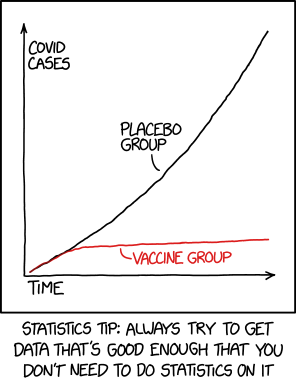
\includegraphics[width=0.6\textwidth,height=0.7\textheight,keepaspectratio]{images/2400_statistics.png}
\end{center}

\bottomnote{XKCD \#2400 by Randall Munroe (CC BY-NC 2.5)}
\end{frame}

\end{document}
